You broach the fog, and the Everloyal follow in your wake. The group passes through a rough-hewn opening and into a large, underground chamber supported by two rows of stone pillars. At the far end of this chamber, its walls give way to a loading dock. A vessel is tied there, bobbing gently against its mooring. Your means of escape has finally presented itself.\\

What little light filters into this place catches off a massive haunch moving through the fog and darkness. Triple the size of the largest warhorse, this beast’s stature is so great that at first it escaped your notice--seemingly part of a pillar or some other architectural feature.\\

“Snickersnee... hee hee...”\\

The beast's form is... familiar, and yet unbeholden to any one animal; as if it were the product of a carnal union between boar, wolf, and shark. It snuffles through the corpses of two dozen guards, using its tusks to jostle them about. Arrows, bolts, and spear shafts protrude from its fur and gills like a pincushion, but the guards’ assault seems to have affected it very little. And though no one speaks, you can feel waves of doubt washing over the Everloyal. Can His faithful succeed where an army of their captors so thoroughly failed?\\

Sinecure Petanti steps backwards, striking his foot against a puddle. And the beast turns suddenly, its roar undulating throughout the cavern. The Everloyal scatter for cover as it comes charging straight towards you.

\subsection*{Victory Condition}
Defeat the Auroks

\subsection*{Doom Events}
\begin{itemize}
\item \textbf{Round 5:} \emph{The Auroks roars and paws at the ground. Its movements are growing more frantic.} The Auroks gains 1 Move value.
\item \textbf{Round 7:} \emph{The Auroks bristles and foams at the mouth.} The Auroks gains 1 of each Defense value.
\item \textbf{Round 9:} \emph{The Auroks lets out a vicious roar.} Increase the damage (if any) of the Auroks’ attacks by 1.
\end{itemize}

\pagebreak

\subsection*{Assist Table}
Once per Round, the player may use a Free action to activate an assist. When activating an assist, cover that entry with a token. That entry is exhausted for the entire encounter, and may not be activated again. Some assists may only be activated if the player possesses their required note.
\begin{tcolorbox}
\begin{center}
\begin{tabular}{ L | L | L }
\multicolumn{1}{c|}{\textbf{Boon of Fire}} & 
\multicolumn{1}{c|}{\textbf{Practical Application}} & 
\multicolumn{1}{c}{\textbf{Furred Distraction}} \\
Gain 1 Enhanced Weapon: Burn (2) condition token\newline \ \newline &
Deal 4 Magic ranged damage to the Auroks\newline \ \newline &
Inflict \emph{Inevitable} Knockdown on the Auroks\newline \ \newline \\
\hline
\multicolumn{1}{c|}{\textbf{Secret Parable}} & 
\multicolumn{1}{c|}{\textbf{Unspoken Word}} &
\multicolumn{1}{c}{\textbf{Snickersnee}} \\
Clear 3 \textbf{HP} slots on the status sheet and gain 1 Enhanced Defense: \textbf{P.DEF} (1) condition token \vfill &
\emph{Requires note c325a}\newline \newline \emph{Reaction.} The character commits a Move 2 \emph{Dodge!} at no \textbf{SP} cost &
\emph{Requires note c322a}\newline \newline The Auroks loses all Defense values for this Round \vfill \\
\end{tabular}
\end{center}
\end{tcolorbox}

\subsection*{Encounter Table}
\begin{tcolorbox}
\textbf{Roll:} 2D6
\begin{center}
\begin{tabular}{ L | L | L }
\multicolumn{1}{c|}{\textbf{2}} & 
\multicolumn{1}{c|}{\textbf{3}} & 
\multicolumn{1}{c}{\textbf{4-5}} \\
\emph{Sudden. Vicious Roar} &
\textbf{A:} \emph{Hind Kick}\newline \textbf{B:} Move.  \emph{Pounce}&
\textbf{A:} \emph{Gore. Gore}\newline \textbf{B:} \emph{ Frenzied Charge} \\
\hline
\multicolumn{1}{c|}{\textbf{6}} & 
\multicolumn{1}{c|}{\textbf{7}} & 
\multicolumn{1}{c}{\textbf{8}} \\
\textbf{A:} \emph{Pounce}\newline \textbf{B:} Move. \emph{Gore} &
\textbf{A:} \emph{Sudden. Hind Kick}\newline \textbf{B:} Move. \emph{Gore. Gore} &
\textbf{A:} \emph{Pounce}\newline \textbf{B:} Move. \emph{Gore} \\
\hline
\multicolumn{1}{c|}{\textbf{9-10}} & 
\multicolumn{1}{c|}{\textbf{11}} & 
\multicolumn{1}{c}{\textbf{12}} \\
\textbf{A:} \emph{Gore. Gore}\newline \textbf{B:} \emph{Frenzied Charge} &
\textbf{A:} \emph{Hind Kick}\newline \textbf{B:} Move.  \emph{Pounce} &
\emph{Sudden. Vicious Roar} \\
\end{tabular}
\end{center}
\end{tcolorbox}

\pagebreak

\subsection*{Enemy Sheets}
\hrule
\ \\
{\large \textbf{The Auroks}}\\\\
\begin{tabular}{s s s}
\textbf{HP:} 45 & \textbf{Move:} 3\\
\textbf{P.DEF:} 2 & \textbf{F.DEF:} 2 & \textbf{M.DEF:} 2 \\
\textbf{L.DEF:} 2 & \textbf{D.DEF:} 2 & \textbf{RES:} 2 \\
\end{tabular}\\

\emph{Large:} This entity occupies two distinct tiles, represented by head and tail tokens. For the purposes of movement, the head tile is moved first and the tail tile is filled-in behind the head, opposite its movement or attack direction. Turning (i.e: just moving the tail) will still use a point of Move.\\

\emph{Great Foe:} This entity ignores all conditions (including Knockback and Knockdown) inflicted by normal sources, except for Blazing and Bleeding, and is immune to Backstab.\\

\emph{Tottering:} If this entity assigns 10 damage tokens to its \textbf{HP} in a single Turn, it is inflicted with Knockdown and Stun upon assigning the tenth token.\\

\textbf{Attacks:}
\begin{itemize}
\item \emph{Gore} -  Move 1. Deal 3 \emph{Unparryable} Pierce damage to an adjacent entity (from head tile).
\item \emph{Pounce} - Move 2. Deal 4 \emph{Unparryable} Crush damage and Knockdown in a half-moon pattern (from head tile).
\item \emph{Hind Kick} - Deal 4 \emph{Unparryable} Crush damage, Knockback 2, and Knockdown to an adjacent entity (from tail tile).
\item \emph{Frenzied Charge} - Move towards the character in a straight or snaking line, until the Auroks attempts to Move onto an impassable tile (including the character’s position). If the character’s position is encountered during this movement, inflict 5 \emph{Unparryable} and \emph{Undodgeable} Pierce damage, Knockback 3, and Knockdown to the character. The Auroks may freely turn one hex before charging.\newline \emph{Always resolve this attack, regardless of whether it will strike the character.}
\item \emph{Vicious Roar} - Inflict \emph{Inevitable} Flinch on all hexes within 3 tiles (from head tile).
\end{itemize}

\begin{tcolorbox}
\textbf{Hint:} While \emph{Charge} deals \emph{Undodgeable} damage, the character may still get out of the way using their reaction’s implicit Move value
\end{tcolorbox}

\pagebreak

\subsection*{Encounter Map}
\begin{center}
\framebox{
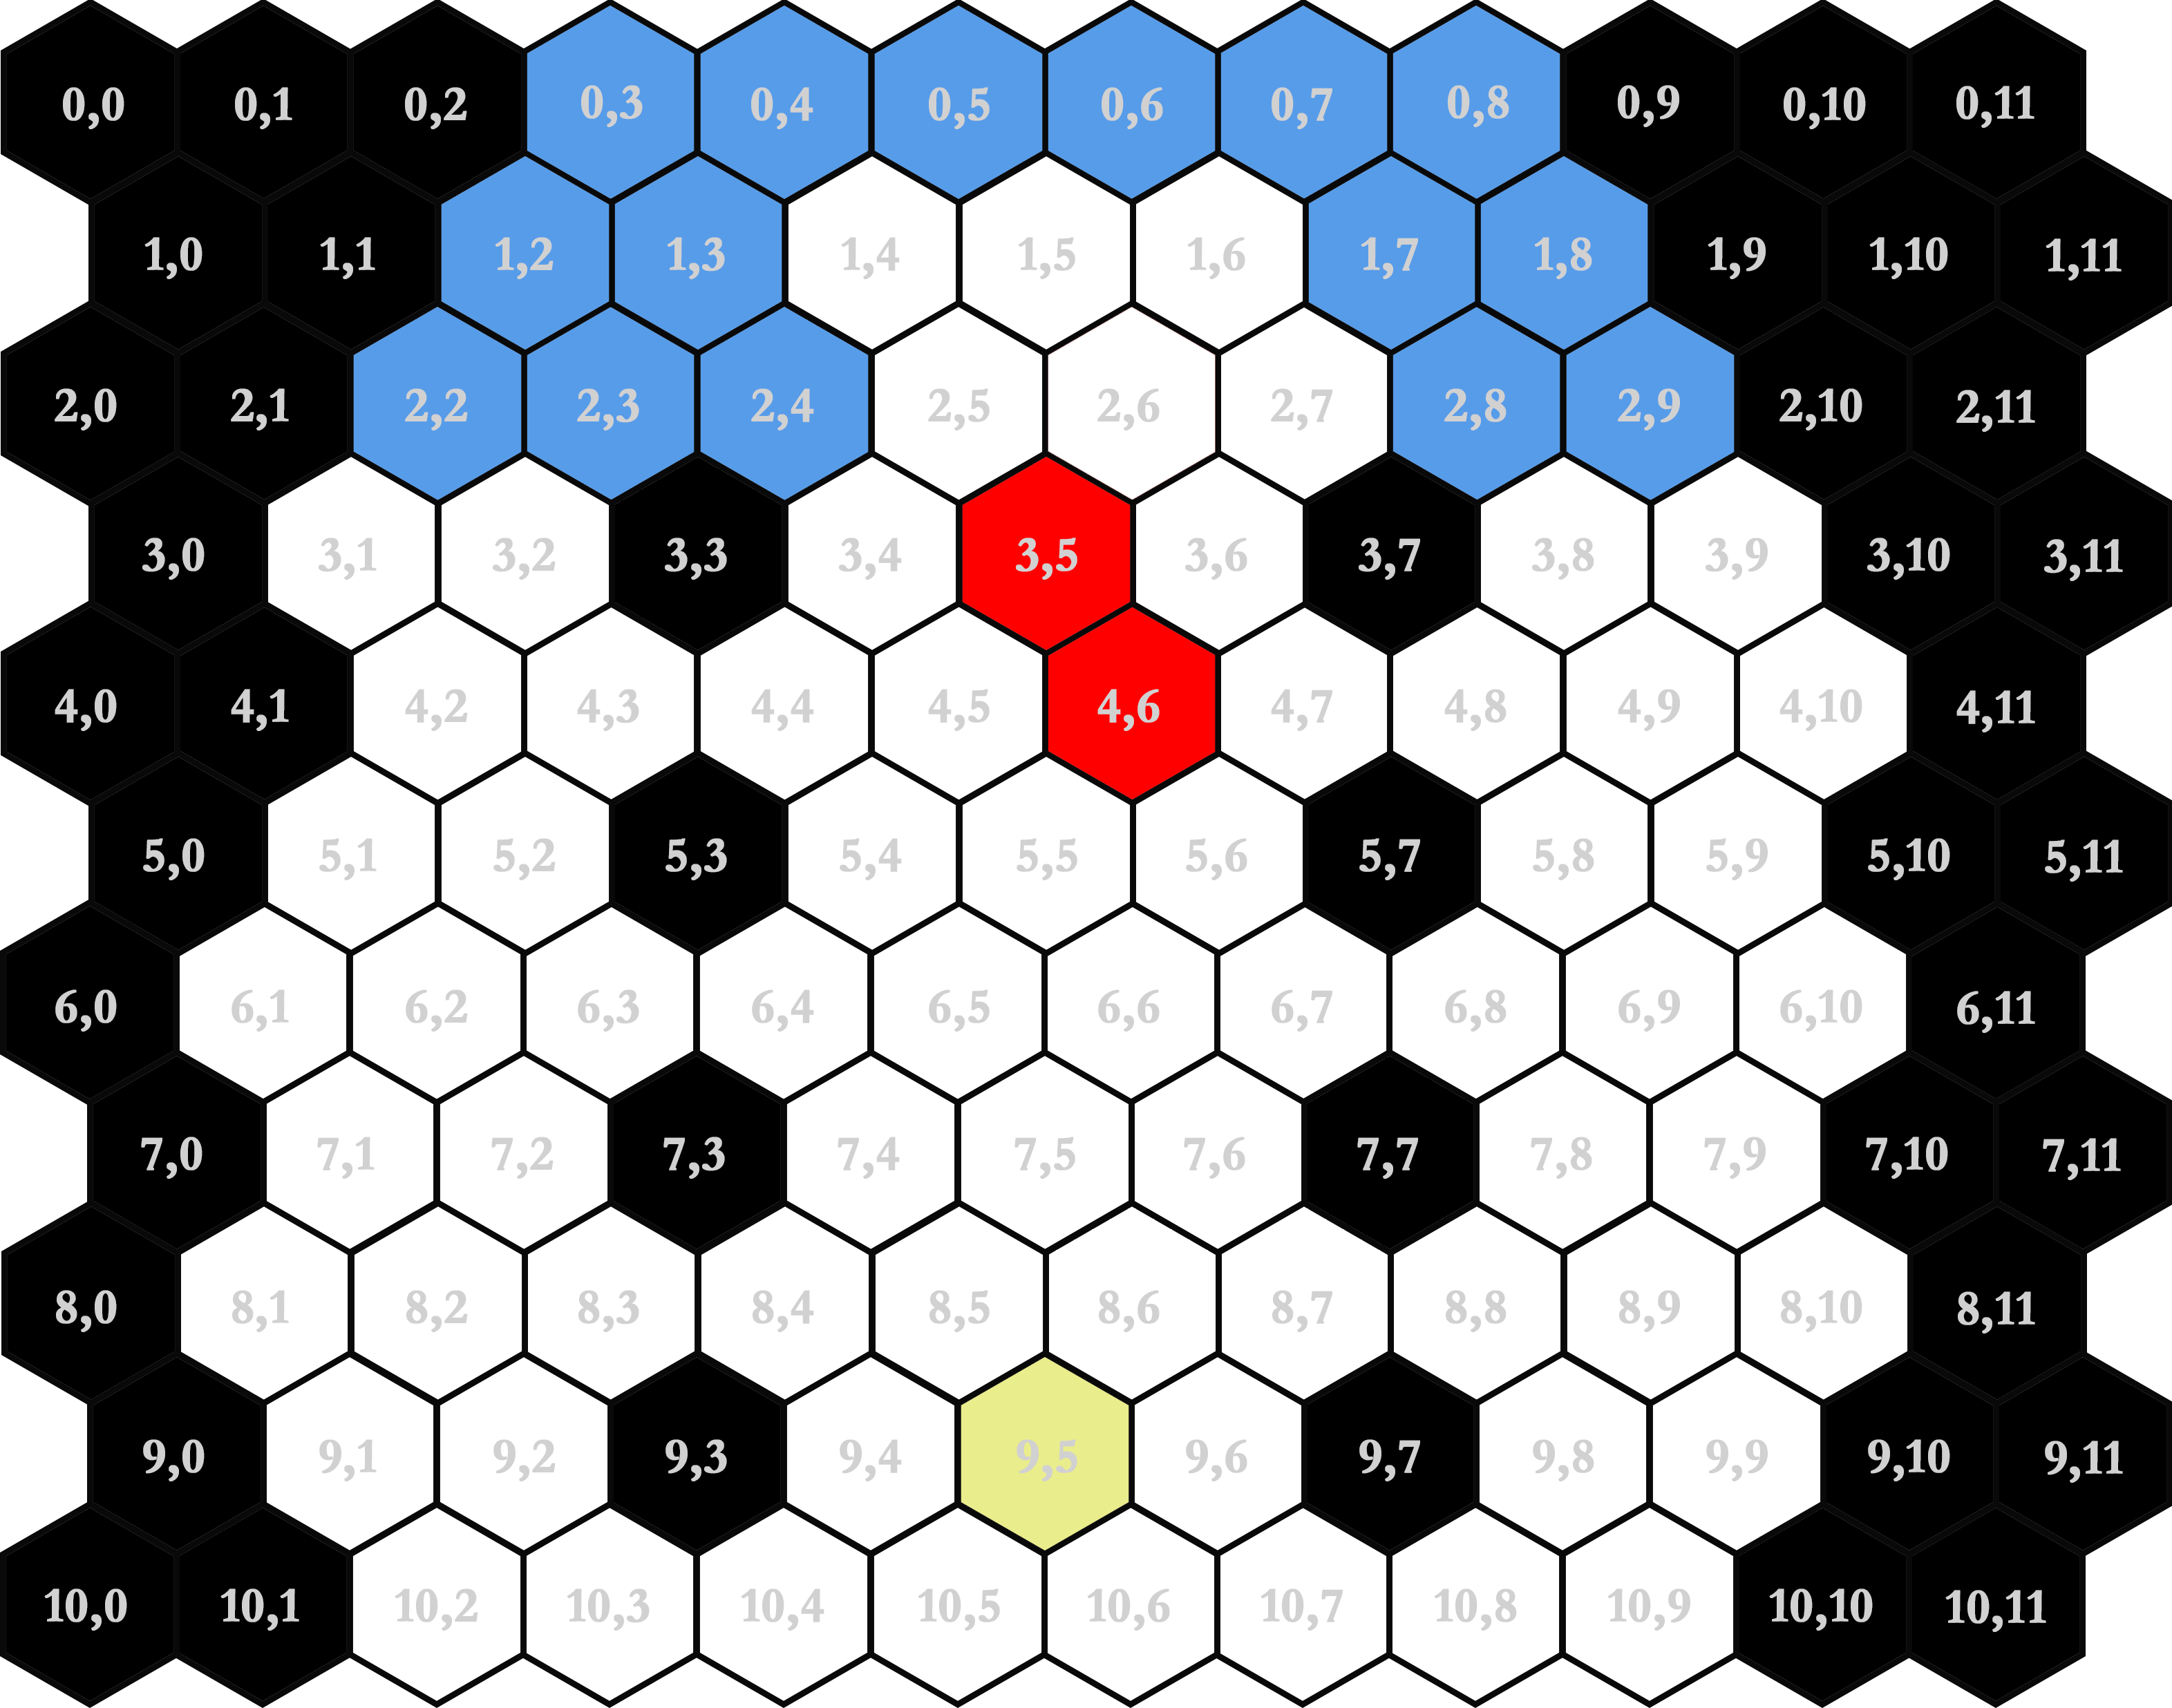
\includegraphics[width = 0.96\textwidth]{./maps/c320.png}
}
\end{center}

\subsection*{Setup Instructions}
\begin{itemize}
\item \textbf{Goldenrod:} Character Start Location. Place the character on either tile.
\item \textbf{Red:} Enemy Start Location. Place the Auroks on these tiles (head on 4,6).
\item \textbf{Blue:} Deep Water. If the character enters this tile, they are defeated.
\item \textbf{Black:} Impassable Boundary/Full-Cover
\end{itemize}

\pagebreak

\subsection*{Victory}
The beast is frantic in death: a wailing, panicked thing. Despite its monstrous appearance it is still a mortal animal, and very much capable of fear. Great gushers of blood spill from its many vorpal wounds, displacing the sea water in the cavern's divots. And with one last cry it sinks down into a great, red pool of itself.\\

Vagabond Lor appears at your side, a large cleaver in his hand. Something pilfered from the kitchen, perhaps. He runs his thumb along its edge, and then approaches the beast in careful, plodding steps.\\

The Auroks cranes its neck to stare. The vagabond’s reflection grows larger in its wild eyes. Its breaths come panicked and labored; its gills open and close, sending sputters of blood across the rough stone floor.\\

And, hefting his cleaver with both hands, Lor does the Auroks a great mercy.\\

>> Soul of a Great Beast (40)\\
>> \textbf{HMN} + 1\\
>> \turnto{c41x1}

\subsection*{Defeat}
As your vision fades you can hear the Everloyal strike up a great panic. Their champion has fallen, and they cannot seem to place this event as part of His machinations.\\
>> \turnto{c41x2}